%!TEX root = ../dissertation.tex
% Insert PDF
% ex. 
\includepdf{figures/inserts/ch6.pdf}

\addthumb{\thechapter}{\Large{\thechapter}}{white}{chaptergrey}
\stopthumb


\includepdf{figures/inserts/ch8.pdf}

% Set chapter number color to be similar to the insert color
\definecolor{chaptergrey}{rgb}{0.203063, 0.379716, 0.553925}

\chapter{Appendix}


\clearpage

\continuethumb

\section{English Summary}

\subsection{Glycosylation}

Each cell in our body is a specialized factory with defined functions: brain cells secrete substances which are important for brain function, immune cells secrete compounds important for cellular communication and antibodies to protect us from dangers from outside the body, and pancreatic cells secrete, among others, insulin to help regulate blood sugar levels.

Within each cell exists a network of interconnected machines, also known as organelles. The organelle central to secretion is the Golgi apparatus, or the Golgi. The Golgi is an important distribution center that receives newly synthesized proteins from the endoplasmic reticulum, performs quality control and final modifications to assert their function and stability, and finally sends them to the proper location inside or outside the cell. In humans, the Golgi consists of a stack of distinct Golgi layers, each with their own roles in these modifications. Similar to man-made distribution centers, having the right materials and products at the right time and right location is of critical importance for optimal Golgi function.

An important modification performed by the Golgi is the attachment of distinct sugars to proteins; this process is called glycosylation\cite{moremen_vertebrate_2012}. These attached sugars, also known as glycans (Figure~\ref{fig:ch8fig1en}) when the structure is complete, make sure that these proteins have the correct structure, function, stability and mode of transport. The Golgi environment, including the acidity inside the Golgi and the localization of all proteins involved in Golgi processes, is precisely regulated to make sure all processes run well. Impairments in the cells that may affect the Golgi or glycosylation result in various diseases that can influence one or more organs.

\begin{figure}
    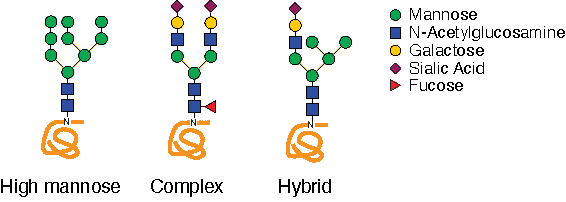
\includegraphics[keepaspectratio=true,width=\textwidth,height=\textheight]{chapters/chapter8/chapter8_Figure1_en.pdf}
    \caption{\textbf{Some examples of glycans.} Glycans are attached to proteins on the amino acid residue asparagine (N) and can form distinct branched structures. Each separate sugar molecule is incorporated in the glycan structure in a step-by-step fashion.}
    \label{fig:ch8fig1en}
\end{figure}

\subsection{Golgi transport}
Of utmost importance for all transport steps in human cells is the delivery of proteins from organelle to organelle. At the Golgi, these transport steps are mainly executed by means of vesicles. These are small membrane-enclosed sacs in which proteins can be carried. Depending on their content, these vesicles are also assigned their destinations. If these vesicles are not delivered in the right place or at the right time however, the consequences can be severe. In \textbf{chapter 2} I have reviewed the literature of all known genetic variants in genes involved in Golgi transport which also lead to a class of diseases called glycosylation disorders. I have learned from this that many of these genetic variants result in diseases with impaired secretion; communication in the brain is often affected or there are developmental problems of the skin or the function of the liver. Developments improving diagnostics of these type of disorders have strongly improved in recent years, offering us better understanding of how Golgi transport works and how this relates to disease.

An important factor for precise Golgi transport is the acidity within the Golgi itself. Golgi acidity is tightly regulated and ensures that Golgi-localized enzymes function optimally and are at the right location. In \textbf{chapter 2} I identified several genetic variants in proteins involved in Golgi acidity regulation, which lead to glycosylation disorders. To study the effects of these genetic variants on Golgi acidity in detail, I developed a novel method to measure the acidity within organelles by microscopy in \textbf{chapter 3}. By labeling organelle-specific proteins with a special acidity-sensitive fluorescent tag, we can use a specialized microscope to accurately determine the acidity within the cell. Moreover, by synchronizing the transport of the cellular communication protein TNF$\alpha$, I demonstrate that we can accurately monitor the acidity of all organelles this protein passes through when it is secreted.

I then applied this novel method in \textbf{chapter 4} to study the function of possible Golgi acidity regulator TMEM199. I found genetic variants in TMEM199 in \textbf{chapter 2} that lead to glycosylation disorders and decreased liver function, but the precise mechanism for these symptoms was not determined. I developed TMEM199-deficient cells using CRISPR/Cas9 and next measured acidity within these cells using the method from \textbf{chapter 3} as well as performed analyses of glycosylation. From these experiments I could conclude that TMEM199 is at least partly responsible for the regulation of Golgi acidity and it does so in concert with the other acidity-regulating protein CCDC115.

\subsection{Syntaxin-5, the most important SNARE protein for Golgi transport}
For each cellular transportation step the fusion of a vesicle with another vesicle or the destination organelle is of absolute importance. In the case of Golgi transport, this implies that the lipid membranes of the vesicle and the Golgi fuse. This process requires the action of members of the SNARE protein family, of which humans have 36 different species. For successful membrane fusion, a complex of four SNARE proteins is necessary; these ensure that the vesicle membrane and organelle membrane merge properly. Specific combinations of SNARE proteins result in unique SNARE complexes for each transport step. This is especially the case for Golgi transport. Transport to, from and within the Golgi is mediated by unique SNARE complexes with one constant member: the SNARE protein syntaxin-5.

Syntaxin-5 exists as a short form and a long form in humans; however, it is still unclear why these two forms exist. In \textbf{chapter 5} I reviewed the literature to find differences and similarities in syntaxin-5 between both humans and yeast, to understand how the function of the protein has changed during evolution. Yeast only expresses one form of syntaxin-5, which we now understand compares best to the long form in humans, but yeast does not have the same layered Golgi structure humans do have.

Subsequently in \textbf{chapter 6}, I discovered in collaboration with colleagues a new genetic variant in syntaxin-5 leading to severe disease with infant mortality. This genetic variant is very rare (three patients were identified in total) and results in expression of only the long form of syntaxin-5. Using patient skin cells with this genetic variant I determined that the organization of and transport around the Golgi is strongly affected. Using specialized experiments, I next observed that the long form of syntaxin-5 is trafficked differently through the cells than the short form and that, ultimately, the short form is more important for transport within the Golgi. Taken together these observations deliver an explanation for the observed disease in these patients.

\subsection{Conclusion}

In my thesis I researched the molecular mechanisms that are the basis of two unique disorders of glycosylation. By means of a novel microscopy method that I developed I have shown that the loss of TMEM199 affects the acidity of the Golgi resulting in impaired glycosylation. Moreover, I have described a novel and rare disorder of glycosylation caused by the loss of syntaxin-5, leading to many separate symptoms and infant mortality. I have discovered that this is due to defective Golgi organization and impaired transport processes around the Golgi.

In summary, this thesis describes how logistics within the cell are important for glycosylation and how glycosylation is affected by impairments in these logistics. The acquired knowledge from this thesis can now be applied to design fitting therapeutic strategies, not only for patients with similar glycosylation disorders, but also for patients with different defects in cellular transportation.

\cleartoleftpage

\section{Nederlandse Samenvatting}

\subsection{Glycosylering}

Elke cel in ons lichaam is een gespecialiseerde fabriek met duidelijke functies: hersencellen scheiden stoffen uit die belangrijk zijn voor de hersenfunctie, immuuncellen scheiden signaleringsstoffen en antilichamen uit om ons te beschermen tegen gevaren van buitenaf, en alvleeskliercellen scheiden onder andere insuline uit ten behoeve van het reguleren van de suikerspiegel.

Binnen elke cel bestaat een netwerk van aaneengekoppelde machines, ook wel organellen genoemd. Het organel dat centraal staat in het uitscheidingsproces is het Golgicomplex, of de Golgi. De Golgi is een belangrijk distributiecentrum dat nieuw gemaakte eiwitten ontvangt van het endoplasmatisch reticulum, vervolgens de kwaliteit controleert en nog laatste aanpassingen voor de stabiliteit en functie uitvoert, en deze eiwitten naar de goede locatie binnen of buiten de cel stuurt. In de mens heeft de Golgi een gelaagde structuur. Net als bij door de mens vervaardigde distributiecentra is het van groot belang dat alle materialen en producten op het juiste moment op de juiste plaats zijn voor optimale werking van de Golgi.

Een belangrijke aanpassing die de Golgi uitvoert is het toevoegen van verschillende suikers aan eiwitten; dit proces wordt glycosylering genoemd\cite{moremen_vertebrate_2012}. Deze toevoegde suikers, die als structuur ook wel glycanen (Figuur 1) heten, zorgen ervoor dat deze eiwitten de goede vorm, functie, stabiliteit, en vervoer hebben. De omgeving binnen de Golgi is heel precies ingesteld, van de zuurgraad tot alle eiwitten die betrokken zijn bij Golgiprocessen. Afwijkingen in de cel die effect hebben op de Golgi of op glycosylering leiden tot verscheidene ziektebeelden die een of meerdere organen kunnen beïnvloeden.

\begin{figure}
    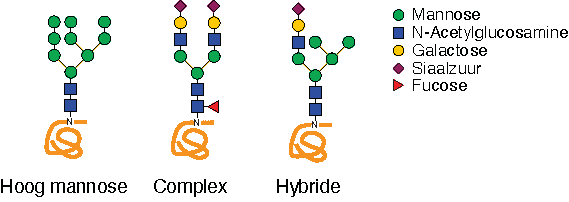
\includegraphics[keepaspectratio=true,width=\textwidth,height=\textheight]{chapters/chapter8/chapter8_Figure1_nl.pdf}
    \caption{\textbf{Enkele voorbeelden van glycanen.} Glycanen worden op eiwitten op het aminozuur asparagine (N) gezet en kunnen verschillende vertakte structuren vormen. De verschillende suikers worden één voor één in de glycaanstructuur gebouwd.}
    \label{fig:ch8fig1nl}
\end{figure}

\subsection{Golgi transport}

Van uiterst belang voor alle transportstappen in menselijke cellen is de aflevering van eiwitten van organel naar organel. Rond de Golgi worden deze transport stappen voornamelijk uitgevoerd met behulp van blaasjes. Dit zijn kleine membraan-omgeven zakjes waarin eiwitten vervoerd kunnen worden. Afhankelijk van de inhoud krijgen deze blaasjes ook hun bestemming toegewezen. Als deze blaasjes echter niet op tijd of op de verkeerde bestemming aankomen, dan heeft dit hevige ziektebeelden als gevolg. In \textbf{hoofdstuk 2} heb ik in de literatuur gekeken naar alle bekende mutaties in genen betrokken bij Golgi transport die ook bekend staan als mogelijke defecten in glycosylering. Hieruit heb ik geleerd dat veel van dit soort mutaties uitmonden in ziektes met beperkte uitscheiding; de communicatie in de hersenen wordt vaak verstoord of er zijn problemen met de ontwikkeling van de huid of de functie van de lever. Ontwikkelingen in de diagnose van dit soort afwijkingen zijn de afgelopen jaren sterk verbeterd en daardoor begrijpen we nu ook beter hoe het transport van de Golgi werkt en ten grondslag ligt aan deze ziektebeelden.

Een belangrijke factor voor nauwkeurig Golgi transport is de zuurgraad binnen de Golgi zelf. Deze zuurgraad is strak gereguleerd en zorgt ervoor dat alle Golgi enzymen zich op de juiste locatie bevinden en dat ze optimaal werken. In \textbf{hoofdstuk 2} heb ik een aantal mutaties gevonden in eiwitten betrokken bij de regulering van de zuurgraad van de Golgi die leiden tot defecten in glycosylering. Om het effect van deze mutaties op de zuurgraad van de Golgi nauwkeurig te kunnen bestuderen, heb ik in \textbf{hoofdstuk 3} een nieuwe methode ontwikkeld om de zuurgraad binnen organellen te meten met microscopie. Door middel van het labelen van specifieke eiwitten in organellen met een zuurgraad-gevoelig fluorescerend label, kunnen we met een speciale microscoop de zuurgraad bepalen in de cel. Daarnaast laat ik in \textbf{hoofdstuk 3} zien dat ik door het synchroniseren van het transport van een bepaald cellulair communicatie-eiwit, TNF$\alpha$, de zuurgraad van alle structuren tijdens het uitscheidingsproces nauwkeuring kan meten.

Deze methode heb ik vervolgens toegepast in \textbf{hoofdstuk 4} om de functie van de mogelijke zuurgraadregulator TMEM199 te bestuderen. In \textbf{hoofdstuk 2} heb ik mutaties gevonden in TMEM199 die leiden tot glycosyleringsdefecten en verminderde leverfunctie, maar het precieze mechanisme hiervan bleek onduidelijk. Ik heb met CRISPR/Cas9 cellulaire modellen ontworpen die TMEM199 missen en vervolgens zowel de zuurgraad in de cel gemeten met de techniek van \textbf{hoofdstuk 3} als analyses op de glycosylering uitgevoerd. Hiervan leerde ik dat TMEM199 in ieder geval ten dele belangrijk is voor de regulatie van de zuurgraad en dit samen met het andere zuurgraad-regulerende eiwit CCDC115 doet.

\subsection{Syntaxin-5, het belangrijkste SNARE-eiwit voor Golgi transport}

Voor elke transportstap in de cel is het van belang dat een blaasje samengaat met een ander blaasje of het organel van bestemming. Voor Golgi transport houdt dit in dat de membranen van het blaasje en de Golgi fuseren. Hiervoor zijn leden van de SNARE-eiwitfamilie nodig, waarvan mensen er 36 verschillende hebben. Voor succesvolle membraanfusie is een complex van in totaal vier SNARE-eiwitten nodig; deze zorgen ervoor dat het membraan van het blaasje en van het organel ineen ritsen. Verschillende combinaties van deze SNARE-eiwitten zorgen ervoor dat unieke SNARE-complexen gevormd worden voor elke transportstap. Dit geldt ook voor Golgi transport. Zowel van en naar, als binnen de Golgi zelf bestaan unieke SNARE-complexen met één constante factor: het SNARE-eiwit syntaxin-5.

Syntaxin-5 bestaat in de mens als een lange vorm en een korte vorm, waarvan nog niet duidelijk is waarom er twee vormen van bestaan. In \textbf{hoofdstuk 5} heb ik in de literatuur gezocht naar verschillen en overeenkomsten in syntaxin-5 tussen de mens en gist, om zo te begrijpen hoe de functie van het eiwit veranderd is tijdens de evolutie. Gist kent namelijk maar één vorm van syntaxin-5, waarvan we nu weten dat het het meeste lijkt op de lange vorm bij de mens, maar dat het niet de gelaagde Golgi structuur bevat die de mens wel heeft.

Vervolgens heb ik in samenwerking met collega’s in \textbf{hoofdstuk 6} een nieuwe mutatie in syntaxin-5 ontdekt die tot hevige afwijkingen van de glycosylering leidt, met babysterfte als gevolg. Deze mutatie is zeer zeldzaam (er zijn in totaal drie patiënten geïdentificeerd) en zorgt ervoor dat alleen de lange vorm van syntaxin-5 geproduceerd wordt. In huidcellen van patiënten met deze mutatie heb ik vastgesteld dat de organisatie van en het transport rondom de Golgi sterk is aangedaan. Met gerichte experimenten heb ik toen gevonden dat de lange vorm van syntaxin-5 anders door de cel beweegt dan de korte vorm en dat de korte vorm belangrijker is voor transport binnen de Golgi. Deze observaties bij elkaar geven een verklaring voor de ziektebeelden van deze patiënten.

\subsection{Conclusie}

In mijn proefschrift heb ik de moleculaire mechanismen onderzocht die ten grondslag liggen aan twee unieke glycosyleringsafwijkingen. Door middel van de ontwikkeling van een nieuwe microscopie methode heb ik laten zien dat het verlies van TMEM199 zorgt voor een verstoring van de zuurgraad in de Golgi met defecte glycosylering als gevolg. Ook heb ik een nieuwe en zeldzame glycosyleringsafwijking beschreven door het verlies van de korte vorm van syntaxin-5, welke leidt tot een breed ziektebeeld en overlijden op jonge leeftijd. Ik heb ontdekt dat dit komt door defecten in de organisatie van de Golgi en transportprocessen rondom de Golgi.

Samenvattend beschrijft dit proefschrift hoe logistieke processen binnen de cel van belang zijn voor glycosylering en hoe de glycosylering aangetast kan worden door afwijkingen in deze logistieke processen. De opgedane kennis uit dit proefschrift kan nu worden gebruikt om passende therapeutische strategieën te ontwerpen, niet alleen voor patiënten met vergelijkbare glycosyleringsafwijkingen, maar ook voor patiënten met andere afwijkingen in cellulair transport.

\cleartoleftpage

\section{Dankwoord}



\cleartoleftpage

\section{Curriculum Vitae (English)}

Peter Linders was born on April 28\textsuperscript{th} 1993 in Oss, the Netherlands. After completing his secondary education in 2011, he started his Bachelor of Sciences degree in Biomedical Sciences at the Radboud University in Nijmegen, the Netherlands. For his Bachelor's internship in 2014, he joined the group of dr. Egbert Oosterwijk at the Department of Experimental Urology at the Radboud Institute for Molecular Life Sciences. Supervised by dr. Marije Sloff and dr. Silvia Mihaila, he investigated the use of adipose-derived stem cells for human urogenital tissue engineering. In 2014, Peter obtained his BSc degree majoring in Human Pathobiology.

Peter continued his education by pursuing a Master of Sciences degree in Biomedical Sciences at the Radboud University with a major in Human Pathobiology. During his first internship in early 2015, he joined the group of prof. dr. Geert van den Bogaart at the Department of Tumor Immunology at the Radboud Institute for Molecular Life Sciences. Under the supervision of Geert and dr. Ilse Dingjan, he worked on the recruitment of NADPH oxidase 2 in dendritic cells. For his second internship in late 2015 and early 2016, he moved to Basel, Switzerland to join the Novartis Institutes for BioMedical Research. Supervised by dr. Emilie Chapeau and dr. Ralph Tiedt, he worked on large-scale experiments to identify new genes involved in cytotoxic T cell activation and exhaustion, using the \emph{piggyBac} transposon system. In 2016, Peter returned to Nijmegen and obtained his MSc degree \emph{bene meritum}.

Using his background in both cell biology and microscopy, Peter started his PhD training in the Membrane Trafficking group of the Tumor Immunology at the Radboud Institute for Molecular Life Sciences in Nijmegen, the Netherlands, supervised by prof. dr. Geert van den Bogaart and prof. dr. Dirk Lefeber. As described in this thesis, he worked on understanding the molecular mechanisms in rare glycosylation disorders. Peter has presented his work at various international conferences and has published several papers in peer-reviewed international scientific journals. During his PhD, Peter has also been an eLife Community Ambassador and was chair of the Radboud Consortium for Glycoscience PhD Council.

\clearpage

\section{Curriculum Vitae (Nederlands)}

Peter Linders werd geboren op 28 april 1993 te Oss. Na het behalen van zijn vwo-diploma in 2011, begon hij met de bachelor Biomedische Wetenschappen aan de Radboud Universiteit Nijmegen. Voor zijn bachelor stage in 2014 sloot hij zich aan bij de onderzoeksgroep van dr. Egbert Oosterwijk bij de afdeling Experimentele Urologie in het Radboud Institute for Molecular Life Sciences. Onder begeleiding van dr. Marije Sloff en dr. Silvia Mihaila, werkte hij aan het gebruik van vetstamcellen in tissue engineering van menselijk urogenitaal weefsel. In 2014, ontving hij zijn BSc diploma met als hoofdvak Humane Pathobiologie.

Peter vervolgde zijn studies door te beginnen aan de master Biomedical Sciences aan de Radboud Universiteit, met een specialisatie in Human Pathobiology. Tijdens zijn eerste masterstage in begin 2015, werd hij deel van de onderzoeksgroep van prof. dr. Geert van den Bogaart bij de afdeling Tumorimmunologie in het Radboud Institute for Molecular Life Sciences. Onder begeleiding van Geert en dr. Ilse Dingjan onderzocht hij het transport van NADPH oxidase 2 naar het fagosoom in dendritische cellen. Voor zijn tweede masterstage eind 2015 tot en met begin 2016 verhuisde hij naar de Novartis Institutes for BioMedical Research in Basel, Zwitserland. Bij de farmacologieafdeling, begeleidt door dr. Emilie Chapeau en dr. Ralph Tiedt, werkte hij aan grootschalige experimenten om nieuwe genen te ontdekken die belangrijk zijn voor cytotoxische T-cel activatie en uitputting, door middel van het \emph{piggyBac} transposon systeem. In 2016 keerde Peter terug naar Nijmegen en ontving hij zijn MSc diploma met het judicium \emph{bene meritum}.

Zijn achtergrond in zowel celbiologie als microscopie toepassend, startte Peter met zijn promotietraject in de Membrane Trafficking onderzoeksgroep van de afdeling Tumorimmunologie bij het Radboud Institute for Molecular Life Sciences, met prof. dr. Geert van den Bogaart en prof. dr. Dirk Lefeber als promotoren. Zoals beschreven in dit proefschrift werkte hij aan het begrijpen van de moleculaire mechanismen in zeldzame glycosyleringsafwijkingen. Peter heeft zijn werk bij verscheidende internationale conferenties gepresenteerd en heeft meerdere publicaties in internationale, peer-reviewed wetenschappelijke tijdschriften. Naast zijn promotieonderzoek was Peter ook betrokken als eLife Community Ambassador en tevens voorzitter van het Radboud Consortium for Glycoscience PhD Council.


\cleartoleftpage

\section{List of Publications}

\noindent\textbf{Linders P.T.A.}, ter Beest M., and van den Bogaart G. \\
\textbf{Fluorescence lifetime imaging of pH along the secretory pathway} \\
\emph{Manuscript in submission at ACS Chemical Biology, 2021}

\vspace{\baselineskip}

\noindent\textbf{Linders P.T.A.}, Gerretsen E., Ashikov A., Vals M.-A., Revelo N.H., de Boer R., Arts R., Baerenfaenger M., Zijlstra F., Huijben K., Raymond K., Muru K., Fjodorova O., Pajusalu S., Õunap K., ter Beest M., Lefeber D.J., and van den Bogaart G. \\
\textbf{Congenital disorder of glycosylation caused by starting site-specific variant in syntaxin-5} \\
\emph{Manuscript in submission at Nature Communications, 2021}

\vspace{\baselineskip}

\noindent\textbf{Linders P.T.A.}, Peters E., ter Beest M., Lefeber D.J., and van den Bogaart G. \\
\textbf{Sugary Logistics Gone Wrong: Membrane Trafficking and Congenital Disorders of Glycosylation} \\
\emph{International Journal of Molecular Sciences 21 p. 4654, 2020}

\vspace{\baselineskip}

\noindent\textbf{Linders P.T.A.}, van der Horst C., ter Beest M. and van den Bogaart G. \\
\textbf{Stx5-Mediated ER-Golgi Transport in Mammals and Yeast} \\
\emph{Cells 8 p. 780, 2019}

\vspace{\baselineskip}

\noindent Paardekooper L.M., Dingjan I., \textbf{Linders P.T.A.}, Staal A.H.J., Cristescu S.M., Verberk W.C.E.P. and van den Bogaart G. \\
\textbf{Human Monocyte-Derived Dendritic Cells Produce Millimolar Concentrations of ROS in Phagosomes Per Second} \\
\emph{Frontiers in Immunology 10 p. 1216, 2019}

\vspace{\baselineskip}

\noindent Ashikov A., Nurulamin A.B., Xiao-Yan W., Niemeijer M., Osorio G.R.P., Brand-Arzamendi K., Hasadsri L., Hansikova H., Raymond K., Simon D.V.M.E.H., Pfundt R., Timal S., Beumers R., Biot C., Smeets R., Kersten M., Huijben K., CDG group, \textbf{Linders P.T.A.}, van den Bogaart G., van Hijum S.A.F.T., Rodenburg R., van den Heuvel L.P., van Spronsen F., Honzik T., Foulquier F., van Scherpenzeel M. and Lefeber D.J. \\
\textbf{Integrating glycomics and genomics uncovers SLC10A7 as essential factor for bone mineralization by regulating post-Golgi protein transport and glycosylation} \\
\emph{Human Molecular Genetics 27(17) p. 3029, 2018}

\clearpage

\noindent Dingjan I., \textbf{Linders P.T.A.}, Verboogen D.R.J., Revelo N.H., ter Beest M. and van den Bogaart G. \\
\textbf{Endosomal and Phagosomal SNAREs} \\
\emph{Physiological Reviews 98(3) p. 1465, 2018}

\vspace{\baselineskip}

\noindent Dingjan I.,  \textbf{Linders P.T.A.}, van den Bekerom L., Baranov M.V., Halder P., ter Beest M. and van den Bogaart G. \\
\textbf{Oxidized phagosomal NOX2 complex is replenished from lysosomes} \\
\emph{Journal of Cell Science 130 p. 1285, 2017}

\cleartoleftpage

\section{Research Data Management}
All primary research data that were generated and presented in this thesis during my PhD were archived according to the FAIR (Findable, Accessible, Interoperable and Resuable) principles. All data are stored digitally on a local server of the Tumor Immunology department of the Radboud university medical center (Radboudumc) and experiments are described in the online lab book system Labguru. All data and documents stored on the local server are accessible to the supervisors and associated scientific staff.

The studies involving human participants of Chapter 6 were performed in accordance with the principles of the Declaration of Helsinki, with approval by the Research Ethics Committee of the University of Tartu and Sanquin. All raw and processed data of Chapters 3 and 6 are also available through the open-source repository Zenodo.

\cleartoleftpage

\section{RIMLS Portfolio}

\footnotesize
\begin{table}[h]
\resizebox{\textwidth}{!}{%
\begin{tabular}{llllll}
\hline
\multicolumn{3}{l}{\textbf{\begin{tabular}[c]{@{}l@{}}Name PhD candidate: P.T.A. Linders\\ Department: Tumor Immunology\\ Graduate School: Radboud Institute for Molecular Life Sciences\end{tabular}}} &
  \multicolumn{3}{l}{\textbf{\begin{tabular}[c]{@{}l@{}}PhD period: 01-10-2016 – 31-03-2021\\ Promotor(s): Prof. Dr. G. van den Bogaart, Prof. Dr. D.J. Lefeber\\ Co-promotor(s): Dr. M. ter Beest\end{tabular}}} \\ \hline
\multicolumn{4}{l}{}                                                                                & Year(s)   & ECTS                 \\ \hline
\multicolumn{6}{c}{\textit{\textbf{TRAINING ACTIVITIES}}}                                                                              \\ \hline
\multicolumn{4}{l}{a) Courses \& Workshops}                                                         &           &                      \\
\multicolumn{4}{l}{- Introduction Day Radboudumc}                                                   & 2016      & 0.5                  \\
\multicolumn{4}{l}{- RIMLS Specific Introductory Course}                                            & 2017      & 1.0                  \\
\multicolumn{4}{l}{- Scientific Journalism}                                                         & 2017      & 3.0                  \\
\multicolumn{4}{l}{- Python for Data Science and Machine Learning Bootcamp}                         & 2017      & 1.25                 \\
\multicolumn{4}{l}{- Scientific Integrity}                                                          & 2018      & 1.0                  \\
\multicolumn{4}{l}{- Grant Writing and Presenting for Funding Committees}                           & 2018      & 1.0                  \\
\multicolumn{4}{l}{- Radboud Consortium for Glycoscience PhD Course\textasciicircum{}}              & 2021      & 2.0                  \\ \hline
\multicolumn{4}{l}{b) Seminars \& Lectures}                                                         &           &                      \\
\multicolumn{4}{l}{- Radboud Research Rounds}                                                       & 2016      & 0.1                  \\
\multicolumn{4}{l}{- RIMLS Lunch Meetings (11)}                                                     & 2016-2019 & 1.2                  \\
\multicolumn{4}{l}{- Personal Grant Information Meeting}                                            & 2018      & 0.2                  \\
\multicolumn{4}{l}{- Data Science \& AI Meeting}                                                    & 2019      & 0.1                  \\ \hline
\multicolumn{4}{l}{c) Symposia \& congresses}                                                       &           &                      \\
\multicolumn{4}{l}{-RIMLS PhD Retreat\textasciicircum{}}                                            & 2017-2019 & 2.25                 \\
\multicolumn{4}{l}{- TIL Symposium on Computational Immunology}                                     & 2017      & 0.25                 \\
\multicolumn{4}{l}{- Protein Trafficking in Health and Disease, Hamburg, Germany\textasciicircum{}} & 2017      & 1.25                 \\
\multicolumn{4}{l}{- CHAINS, Veldhoven\textasciicircum{}}                                           & 2017      & 0.75                 \\
\multicolumn{4}{l}{- FEBS Golgi Meeting, Sorrento, Italy\textasciicircum{}}                         & 2018      & 1.75                 \\
\multicolumn{4}{l}{- ASCB|EMBO Meeting, Washington DC, USA\textasciicircum{}}                       & 2019      & 1.75                 \\
\multicolumn{4}{l}{- EUROGLYCANomics Online Meeting\textasciicircum{}}                              & 2020      & 0.75                 \\ \hline
\multicolumn{4}{l}{d) Other}                                                                        &           &                      \\
\multicolumn{4}{l}{- Journal Clubs}                                                                 & 2016-2021 & 6.0                  \\
\multicolumn{4}{l}{- Tumor Immunology Meeting Presentations}                                        & 2016-2021 & 5.0                  \\
\multicolumn{4}{l}{- Manuscript Peer-review}                                                        & 2018      & 0.1                  \\
\multicolumn{4}{l}{- eLife Community Ambassador}                                                    & 2019-2020 & 0.5                  \\
\multicolumn{4}{l}{- Radboud Consortium for Glycoscience PhD Council Chair}                         & 2020-2021 & 3.0                  \\ \hline
\multicolumn{6}{c}{\textit{\textbf{TEACHING ACTIVITIES}}}                                                                                                \\ \hline
\multicolumn{4}{l}{e) Lecturing}                                                                    &           &                      \\
\multicolumn{4}{l}{- Biomedical Sciences / Medicine Imaging Minor}                                  & 2017      & 0.3                  \\
\multicolumn{4}{l}{- Biomedical Sciences / Medicine MIN04}                                          & 2018      & 0.5                  \\
\multicolumn{4}{l}{- Biomedical Sciences / Medicine Grant Proposals}                                & 2019-2020 & 1.0                  \\ \hline
\multicolumn{4}{l}{f) Supervision of Internships / Other}                                           &           &                      \\
\multicolumn{4}{l}{- Supervision Master's Students (4)}                                             & 2017-2021 & 7.0                  \\
\multicolumn{4}{l}{- Supervision Master's Thesis (1)}                                               & 2018-2019 & 1.5                  \\
\multicolumn{5}{l}{\textit{\textbf{TOTAL}}}                                                                     & \textit{\textbf{45}}
\end{tabular}%
}
\end{table}

\normalsize